\appendix

\chapter{}

\section{符号说明}
\subsection{通用符号说明}

\begin{table}[H]
    \centering
    \caption{通用输入输出符号}
    \label{table:通用输入输出符号}
    \setlength{\tabcolsep}{3.5mm}
    \begin{threeparttable}
    \begin{tabular}{c|c|cc|c}
        \toprule
        & \textbf{符号} & \textbf{含义} & \textbf{符号} & \textbf{含义}\\
        \midrule
        \multirow{4}*{\makecell{监督\\学习}}& $X$ & 输入变量集合 & $x$ & 输入变量取值 \\
        & $Y$ & 输出变量集合 & $y$ & 输出变量取值 \\
        & $x^{(i)}$ & 输入变量 $x$ 的第 $i$ 个特征值 & $x_i$ & 输出变量集的第 $i$ 个变量 \\
        & $T$ & 输入与输出对/样本点 & & \\
        \midrule
        \multirow{2}*{\makecell{无监督\\学习}}& $\mathcal{X}$ & 输入空间 & $x$ & 输入变量取值 \\
        & $\mathcal{Z}$ & 输出空间 & $z$ & 输出变量取值 \\
        \bottomrule
    \end{tabular}
    \end{threeparttable}
\end{table}

\begin{table}[H]
    \centering
    \caption{监督学习模型符号}
    \label{table:监督学习模型符号}
    \setlength{\tabcolsep}{7mm}
    \begin{threeparttable}
    \begin{tabular}{c|cc|c}
        \toprule
        \textbf{符号} & \textbf{含义} & \textbf{符号} & \textbf{含义}\\
        \midrule
        $\mathcal{F}$ & 假设空间 & $L(Y,f(X))$ & 损失函数 \\
        $R_{exp}$ & 风险函数 & $R_{emp}$ & 经验风险 \\
        $R_{srm}$ & 结构风险 & $J(f)$ & 模型复杂度\\
        \bottomrule
    \end{tabular}
    \end{threeparttable}
\end{table}


\section{重要概念}

\subsection{贝叶斯定理}

\subsubsection{基础概率论}

\noindent\textbf{条件概率公式}

设 $A,B$ 是两个事件,且 $P(B)>0$,则在事件$B$发生的条件下,事件 $A$ 发生的条件概率为:
\begin{equation}
    P(A|B)=\frac{P(AB)}{P(B)}
\end{equation}

条件概率中,事件 $A,B$ 一般是有交集的,否则条件概率为 0 。

\begin{figure}[H]
    \centering
    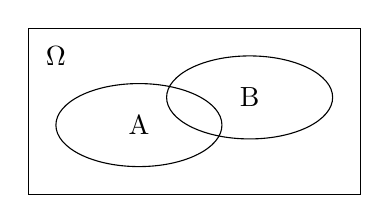
\begin{tikzpicture}[scale = 1]
        \node [draw,inner xsep=6em,inner ysep=3em] at (0,0) {};
        \node at (-5em,2em) {$\Omega$};
        \draw (-2em,-0.5em) ellipse [x radius = 3em, y radius = 1.5em, line width=1pt];
        \draw (2em,0.5em) ellipse [x radius = 3em, y radius = 1.5em, line width=1pt];
        \node at (-2em,-0.5em) {A};
        \node at (2em,0.5em) {B};
    \end{tikzpicture}
    \caption{条件概率}
\end{figure}

\noindent\textbf{乘法公式}

1. 由条件概率公式得乘法公式:
\begin{equation}
    P(AB) = P(A|B)P(B) = P(B|A)P(A)
\end{equation}

2. 乘法公式推广:对于任意正整数 $n\geq 2$,当 $P(A_1A_2\dots A_{n-1})>0$ 时,有:
\begin{equation}
    P(A_1A_2\dots A_{n-1}A_n) = P(A_1)P(A_2|A_1)P(A_3|A_2A_1) \dots P(A_n|A_1A_2\dots A_{n-1})
\end{equation}

\noindent\textbf{全概率公式}

如果事件组 $B_1,B_2,\dots$ 满足如下条件,则称为事件组为样本空间的恶一个划分:
\begin{enumerate}
    \item $B_1,B_2,\dots$ 两两互斥,即 $B_i \cap B_j = \varnothing \quad i \neq j; i,h = 1,2,\dots ; P(B_i)>0$
    \item $B_1 \cup B_2 \cup \dots = \Omega$
\end{enumerate}

则有:
\begin{equation}
    P(A) = \sum_{n=1}^{\infty} P(B_i) P(A|B_i) 
\end{equation}

\subsubsection{贝叶斯定理}

贝叶斯定理是英国数学家贝叶斯提出的,其主要用于解决"逆概率"问题,即在得知概率后,判断条件\footnote{瞎编的}。

将条件概率公式变形得到如下公式:
\begin{equation}
    P(A|B) = \frac{P(B|A)P(A)}{P(B)} = P(A)\frac{P(B|A)}{P(B)}
\end{equation}

定义以下名词:
\begin{enumerate}
    \item 先验概率:$P(A)$,即在不知道B事件的前提下,对A事件概率的主观判断。
    \item 可能性函数:$P(B|A)/P(B)$,作为调整因子,作用是使得先验概率更接近真实值。
    \begin{itemize}
        \item 若 $P(B|A)/P(B)>1$:先验概率增强,事件A发生概率可能性变大。
        \item 若 $P(B|A)/P(B)=1$:事件B无助于判断事件A的可能性。
        \item 若 $P(B|A)/P(B)<1$:先验概率削弱,事件A发生概率可能性变小。
    \end{itemize}
    \item 后验概率:$P(A|B)$,即在事件B发生后对事件A的概率进行重新评估。
\end{enumerate}

\subsubsection{参考文献}
此篇引用的文章如下:
\begin{itemize}
    \item \href{https://blog.csdn.net/qq_31073871/article/details/81077386}{CSDN:基础概率论}
    \item \href{https://blog.csdn.net/qq_41529692/article/details/84105315}{CSDN:贝叶斯公式及其应用}
\end{itemize}

\subsection{最小二乘法}
\subsubsection{最小二乘法原理}

最小二乘法核心思想:如果误差是随机的,应该围绕真值上下波动。

假设 $y$ 表示真值,$y_i$表示样本值,就有最小二乘法:

\begin{equation}
    \epsilon = \sum(y-y_i)^2 \text{最小} \Longrightarrow \text{真值} y
\end{equation}

\subsubsection{最小二乘的应用}

在机器学习领域中,可以将真值看作模型函数 $y=f(x_i)$, 样本看作输出 $y_i$,那么就有:

\begin{equation}
    \epsilon = \sum(f(x_i)-y_i)^2
\end{equation}

再结合多元微积分\footnote{这部分内容可能超过了理工科通修的数学体系}的知识,就可以求解。

\subsubsection{参考文献}
此篇引用的文章如下:
\begin{itemize}
    \item \href{https://blog.csdn.net/ccnt_2012/article/details/81127117}{CSDN:如何理解最小二乘法}
\end{itemize}